\chapter{Infraestructura}\label{cap.infraestructura}
En este capítulo se describen las tecnologías sobre las que se cimenta este trabajo. Se empezará haciendo una introducción al mundo de los robots, ya sean reales o simulados, a los que las herramientas que se van a desarrollar en este trabajo podrán conectarse. Posteriormente se indican las diferentes infraestructuras de robótica y comunicación utilizadas en el desarrollo de este trabajo, destacando la plataforma JdeRobot y los \textit{middleware} de comunicación ICE y ROS. Finalmente, se explican diferentes infraestructuras de tecnologías web, haciendo especial hincapié en el entorno Electron y Node.js, ya que se dotará a todas las herramientas desarrolladas la posibilidad de ser ejecutadas por estas dos vías.

\section{Robots reales y simulados}
Los robots pueden ser reales o simulados. Mientras que los robots reales son más costosos y más difíciles de manejar, los robots simulados permiten que cualquier persona desde un ordenador pueda probar sus desarrollos sin riesgo y que posteriormente sean capaces de funcionar con un robot real.

Las herramientas desarrolladas en este trabajo son capaces de conectarse a los robots, tanto simulados como reales.

\subsection{Robots simulados: Gazebo}
Se trata del principal programa de simulación de robots existente\footnote{\url{http://gazebosim.org/}}, de código abierto y bajo la licencia Apache 2.0, que lleva largo tiempo utilizándose en laboratorios de investigación de robótica e inteligencia artificial. Con Gazebo es posible simular desde una cámara a robots más complejos de una forma sencilla gracias a su interfaz simple e intuitiva. Cada robot cuenta con drivers simulados como pueden ser la cámara, los sensores o los actuadores, de manera que la experiencia sea lo más parecida a un robot real.

En este trabajo se va a hacer un uso destacable de este simulador en su version 7.14, conectando cada uno de los visores a un robot simulado. En concreto, las herramientas son capaces de conectarse a un Turtlebot (Figura 3.1) y un drone simulados obteniendo la información o enviando órdenes a los diferentes drivers del robot: la cámara, el láser y los motores.

\begin{figure}[H]
  \begin{center}
    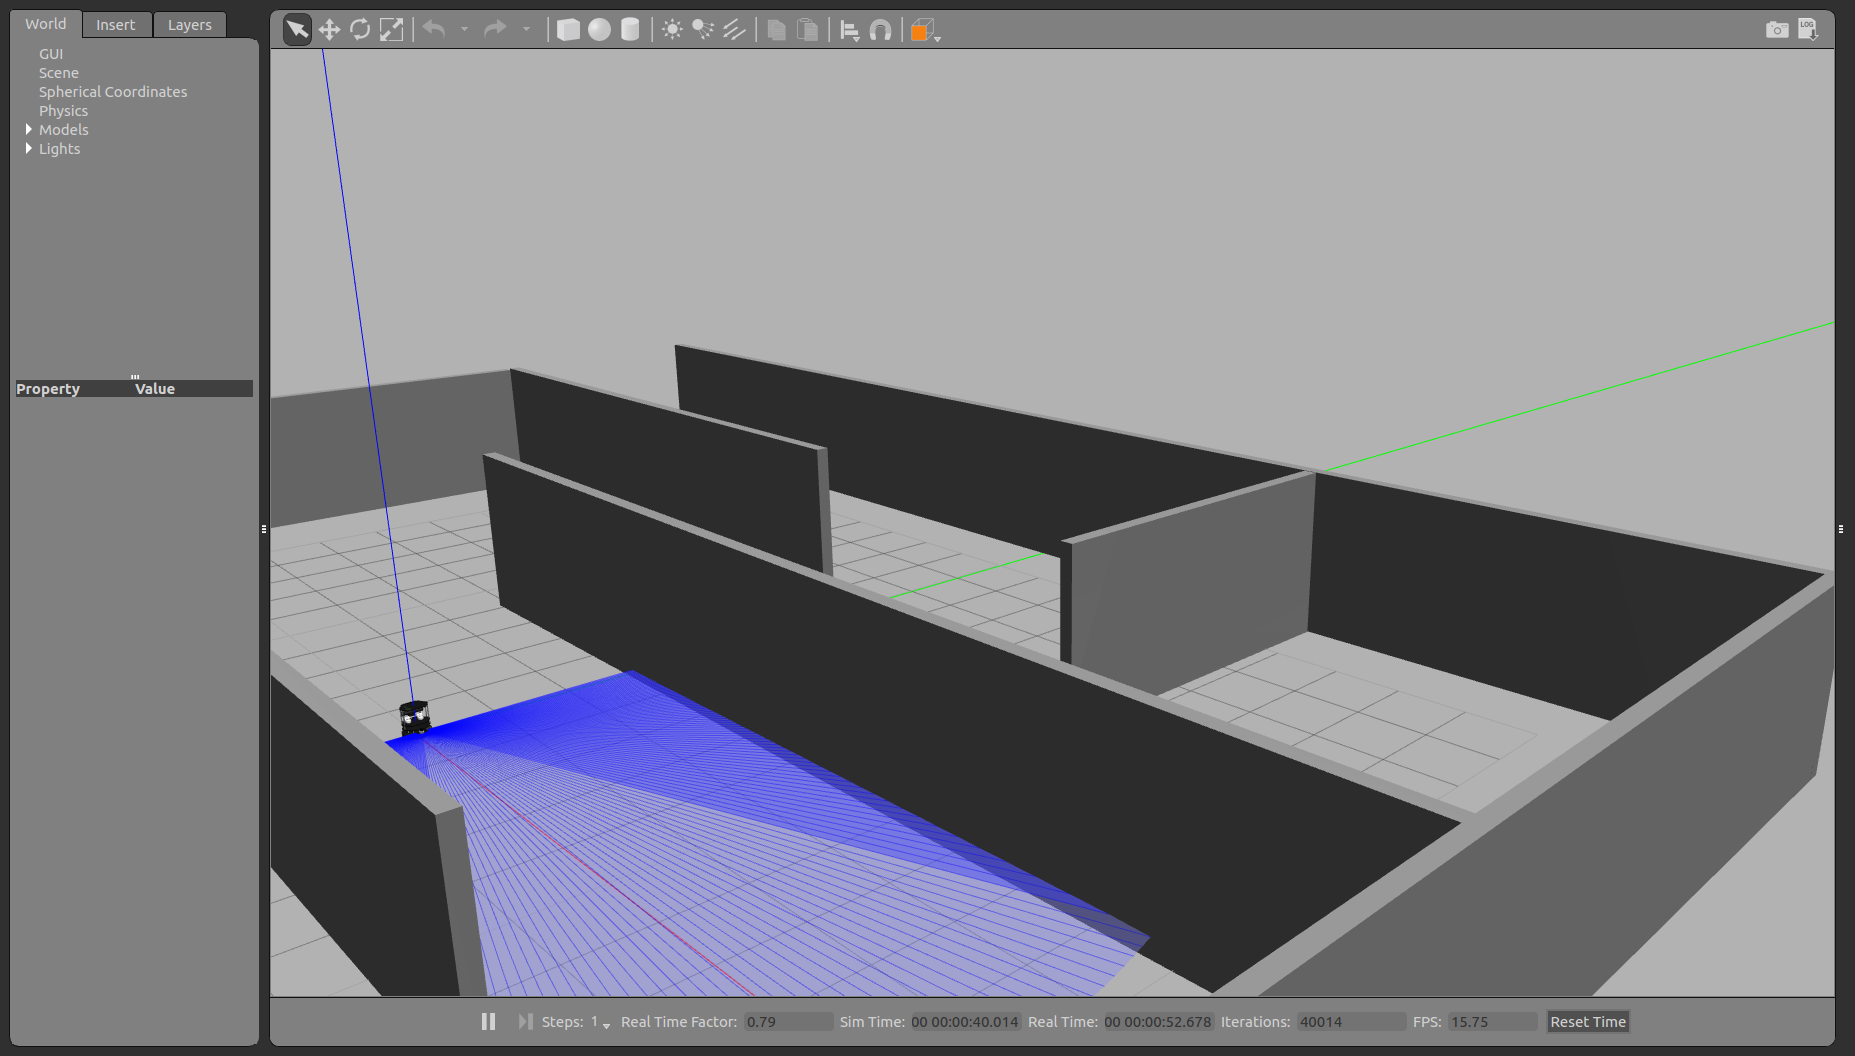
\includegraphics[width=0.8\textwidth]{figures/gazeboturtle.png}
		\caption{Robot Turtlebot simulado con Gazebo}
		\label{fig.robotsimulado}
		\end{center}
\end{figure}

\subsection{Robots reales}
Gracias a que las herramientas elaboradas se han probado con los robots simulados durante el desarrollo, es posible probarlas con robots reales sabiendo que las herramientas van a funcionar correctamente. Tanto el robot Turtlebot real (Figura 3.2) como el drone real, cuentan con los mismos drivers que sus versiones simuladas, por lo que la información obtenida o las órdenes transmitidas será la misma y las herramientas podrán conectarse sin ningún tipo de problema.

\begin{figure}[H]
  \begin{center}
    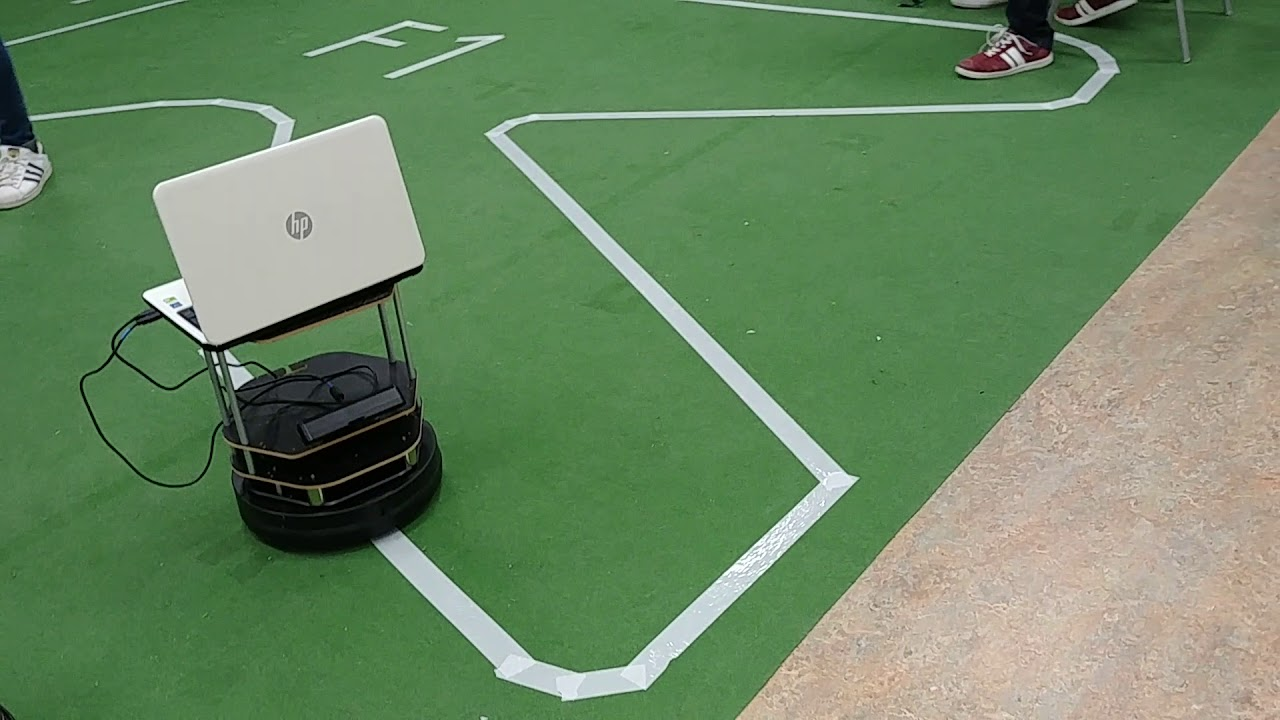
\includegraphics[width=0.8\textwidth]{figures/turtlebotreal.jpg}
		\caption{Robot Turtlebot real}
		\label{fig.robotreal}
		\end{center}
\end{figure}


\section{La plataforma JdeRobot}
JdeRobot\footnote{\url{https://jderobot.org/Main_Page}} es un entorno de software libre para robótica y visión artificial creado por el grupo de robótica de la Universidad Rey Juan Carlos y licenciado bajo GPL v3\footnote{\url{http://www.gnu.org/licenses/gpl-3.0-standalone.html}}. Su desarrollo principalmente está realizado mediante C, C++ y Python, incorporando últimamente desarrollos en JavaScript, como en este trabajo.

JdeRobot está basado en componentes que son interconectados mediante el uso de middlewares como ICE o ROS, facilitando el acceso a los dispositivos hardware. Estos componentes obtienen mediciones  de los sensores u órdenes del motor a través de llamadas a funciones locales. JdeRobot conecta esas llamadas a drivers conectados a sensores (para la recepción de las mediciones) o actuadores (para las órdenes), ya sean reales o simulados. Estas funciones locales forman la API de la capa de abstracción del hardware (HAL-API). La plataforma también ofrece una serie de herramientas para facilitar la teleoperación o el procesamiento de las mediciones de los sensores, y bibliotecas.

Para el desarrollo de este proyecto, se ha usado la versión de JdeRobot 5.6.4

\section{El Middleware ICE}
Se trata de una biblioteca orientada a objetos que ayuda a crear aplicaciones distribuidas fácilmente\footnote{\url{https://zeroc.com/}}. ICE se ocupa de todas las interacciones con las interfaces de programación de bajo nivel de red (ahorra al desarrollador la tarea de apertura de puertos, conexiones de red o serialización de datos). El objetivo principal de ICE es facilitar el desarrollo de aplicaciones, de modo que en muy poco tiempo se pueda aprender a utilizarlo. Toda conexión ICE cuenta con un cliente y un servidor, de modo que el cliente siempre lleva la iniciativa de la conexión, enviando peticiones al servidor, el cual responde a esas peticiones. En la Figura 3.3 puede verse esta estructura de cliente-servidor.

\begin{figure}[H]
  \begin{center}
    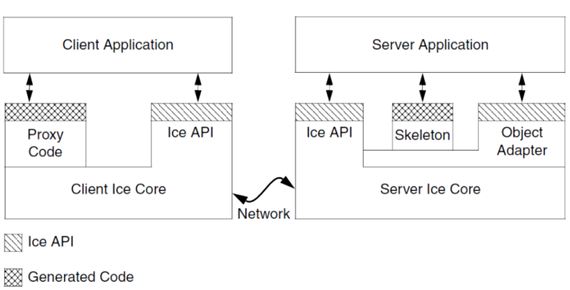
\includegraphics[width=0.8\textwidth]{figures/estructuraice.png}
		\caption{Estructura de Cliente - Servidor con Ice}
		\label{fig.estructurarice}
		\end{center}
\end{figure}

ICE tiene un lenguaje de especificación propio llamado Slice (Specification Language for ICE) que permite la abstracción fundamental para separar interfaces de objetos de sus implementaciones. Este lenguaje especifica las interfaces, operaciones y tipos de parámetros utilizados por la aplicación. Cada una de las aplicaciones que se deseen que se comuniquen entre sí deben compartir la misma descripción Slice. Esta descripción es independiente del lenguaje en el que está desarrollado nuestro cliente o servidor, de modo que es posible su utilización con clientes y servidores escritos en diferentes lenguajes de programación.

Las interfaces \texttt{Slice} pueden verse como un contrato firmado entre un cliente y un servidor para compartir los mismos tipos, funciones y elementos, dando igual el lenguaje de programación en el que estén escritos, ya que posteriormente se traducen usando el compilador correspondiente al lenguaje de programación respectivo. Si el cliente y el servidor no compartiesen la misma interface \texttt{Slice}, la conexión no podría llevarse a cabo al no conocer las funciones o tipos que maneja cada uno.

Para este trabajo se va a utilizar su versión para JavaScript. El soporte para este lenguaje es relativamente reciente, por lo que muchas de las funcionalidades que ofrece para otros lenguajes de programación como C++ o Python, no están aún disponibles para JavaScript. Por ejemplo no hay soporte para la creación de un servidor completo mediante JavaScript. Por ello durante este trabajo se ha optado por utilizar ICE únicamente como cliente, con las ventajas e inconvenientes a los que se hará referencia en próximos capítulos.

La versión de ICE que se usa en este trabajo para conectar las herramientas web con los drivers robóticos es la 3.6.4.

\section{El Middleware ROS}
Se trata de un ecosistema para el desarrollo de software robótico que ofrece las funcionalidades de un sistema operativo (abstracción del hardware, control de dispositivos de bajo nivel, mantenimiento de paquetes, etc.)\footnote{\url{http://www.ros.org/}}. ROS ofrece una serie de herramientas, bibliotecas y convenciones para simplificar la tarea de crear complejas y robustas aplicaciones para robots. Nace con la idea de fomentar el desarrollo colaborativo, es decir que cualquier persona que realice un desarrollo puede subir a los repositorios que ofrece ROS para ello, de modo que otros puedan reutilizarlo en sus proyectos con relativa facilidad.

El elemento fundamental del funcionamiento de ROS es el nodo. Un nodo es un proceso que realiza cálculos y se comunica con otros mediante: (a) un sistema de publicación - subscripción para conexiones asíncronas y anónimas, o (b) servicios para las conexiones síncronas. 

Típicamente cada nodo se ocupa de una parte del sistema de control de robot, por ejemplo un nodo se ocupa de los motores, otro de realizar la localización, etc. Este elemento proporciona mayor tolerancia a los fallos al ser bloques separados y aislados, y se reduce la complejidad del código.

En el sistema de comunicación asíncrona (Figura 3.4), un nodo actúa como publicador que transmite un mensaje con una etiqueta llamada \textit{topic} por el canal para que sea recibido por cualquier otro nodo que se subscriba a esta etiqueta o \textit{topic}. El mensaje enviado es una estructura de datos simple, que comprende campos tipados. ROS ofrece una serie de formatos de mensajes estándar que cubren la mayoría de necesidades de uso común (mensajes para sensores, cámaras, movimiento, láseres, nubes de puntos, etc).

\begin{figure}[H]
  \begin{center}
    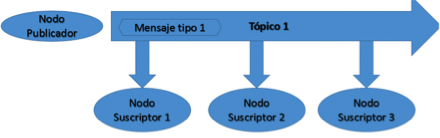
\includegraphics[width=0.8\textwidth]{figures/publicadorsubscriptor.png}
		\caption{Estructura del sistema de comunicación Publicador - Subscriptor}
		\label{fig.publicadorsubscriptor}
		\end{center}
\end{figure}

El sistema de comunicación síncrona (Figura 3.5) es el típico sistema de llamada a procedimiento remoto, a través del cual un nodo ROS es el prestador del servicio que permanece en escucha continua y el resto de nodos le envían mensajes de solicitud. Cada servicio está definido por la cantidad y tipo de datos que necesita, tanto para recibir la petición, como para enviar la respuesta.

\begin{figure}[H]
  \begin{center}
    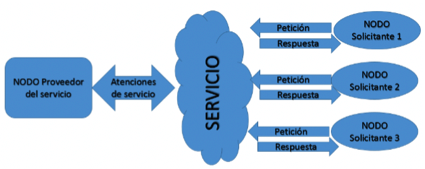
\includegraphics[width=0.8\textwidth]{figures/serviciosros.png}
		\caption{Estructura del sistema de comunicación por Servicios ROS}
		\label{fig.serviciosros}
		\end{center}
\end{figure}

Un elemento muy útil para este proyecto es que ROS proporciona total compatibilidad con Gazebo mediante un conjunto de paquetes llamados \textit{gazebo\_ros\_pkgs} \footnote{\url{http://wiki.ros.org/gazebo_ros_pkgs}}. En ROS, los paquetes son aquellos donde se incluye todo el código fuente, las librerías usadas y cualquier otro recurso necesario para que funcione el nodo.

La versión de ROS que se utilizará para el desarrollo de este trabajo es ROS Kinetic.

\section{Robot Web Tools}
Robot Web Tools\footnote{\url{http://robotwebtools.org/}} es una comunidad nacida a partir de la de ROS, cuyo software permite conectar aplicaciones web a elementos robóticos gracias a un intermediario llamado \texttt{Rosbridge}. Este intermediario es a la vez una especificación de JSON para interactuar con ROS y una capa de transporte para que los clientes se comuniquen mediante WebSockets. 

Por otro lado, han creado una serie de bibliotecas livianas y fáciles de utilizar de JavaScript que proporcionan una abstracción de la funcionalidad principal de ROS. Estas bibliotecas son \texttt{roslibjs}, \texttt{ros2djs} y \texttt{ros3djs}. En este trabajo solo se utiliza \texttt{roslibjs}.

La biblioteca \texttt{roslibjs} se encarga de ofrecer las funcionalidades necesarias para conectar, enviar o recibir mensajes ya sea mediante publicación y subscripción o mediante servicios. La conexión se realiza a un servidor intermedio (\texttt{Rosbridge Server}), el cual se encarga de gestionar las conexiones, los \texttt{topic} publicados o los servicios activos en cada momento, de modo que cuando un nodo se subscriba o realice la petición de un servicio, este servidor contiene la capa de transporte para encaminar la petición mediante WebSockets. La funcionalidad de este servidor intermedio y las interacciones se pueden apreciar en la figura 3.6.

\begin{figure}[H]
  \begin{center}
    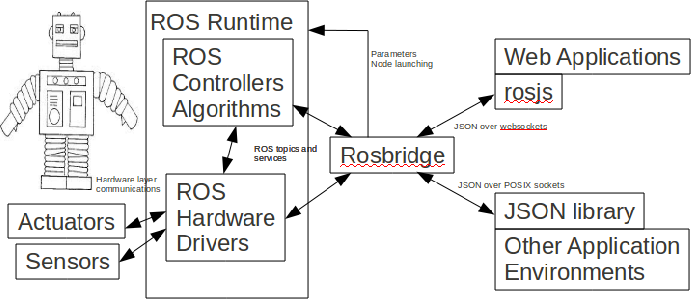
\includegraphics[width=0.8\textwidth]{figures/estructurarosbridge.png}
		\caption{Estructura de una aplicación con Rosbridge}
		\label{fig.estructurarosbridge}
		\end{center}
\end{figure}

Dado que para este trabajo se va a utilizar JavaScript como lenguaje, se utilizará \textit{Rosbrige} en todas las partes relacionadas con ROS, las bibliotecas, servidores y protocolo indicado en esta sección.
\section{Node.js}
Node.js\footnote{\url{https://nodejs.org/es/}} es un entorno multiplataforma del lado del servidor. Concebido con la intención de facilitar la creación de programas de red escalables, como puede ser un servidor web, permite ejecutar código JavaScript fuera de un navegador y aprovechar las ventajas que proporciona su programación orientada a eventos. Su ejecución se lleva a cabo en un único hilo, usando entradas y salidas asíncronas que pueden ejecutarse de manera concurrente, provocando que cada una de ellas necesite de un \textit{callback} para manejar los eventos. 

Node.js proporciona una serie de módulos básicos que permiten realizar funciones esenciales como puede ser la programación en red asíncrona, el manejo de archivos del sistema, etc. Al ser de código abierto, existe una gran comunidad de desarrolladores que crean nuevos módulos para que cualquiera pueda utilizarlos. Estos módulos son fácilmente compartidos gracias al manejador de paquetes npm\footnote{\url{https://www.npmjs.com/}}, permitiéndo compilar, instalar y manejar las dependencias de cualquier módulo de terceros que deseemos usar en nuestro proyecto.
 
Por lo general, un proyecto Node.js contendrá al menos dos elementos, un archivo .js que contendrá la lógica del programa escrita en JavaScript y un segundo archivo llamado Package.json que definirá nuestro programa. Este segundo archivo es donde se indican las dependencias que usará nuestro programa y facilitará su instalación conjunta usando el comando npm install, así como se referenciará al fichero .js indicado anteriormente.

La versión de Node.js utilizada es la 8.9.1 y la versión del manejador de paquetes npm es la 6.4.0.

\section{WebGL y Three.js}
WebGL \footnote{\url{https://get.webgl.org/}}  es un API multiplataforma utilizado para crear gráficos 3D utilizando tecnologías web, está basado en OpenGL y utiliza parte de su API. WebGL se ejecuta dentro del elemento HTML Canvas, lo que proporciona una completa integración con la interfaz DOM. Ofrece ventajas como la compatibilidad con distintos navegadores y plataformas, no es necesario compilar para su ejecución o la interacción con otros elementos del HTML. Sin embargo, debido a que se trata de un API de bajo nivel es complejo de utilizar.

Three.js \footnote{\url{https://threejs.org/}} nace como remedio a la complejidad de usar WebGL. Se trata de una biblioteca desarrollada en JavaScript que permite crear y mostrar gráficos 3D en un navegador web usando un API de alto nivel, proporciona funciones y objetos para facilitar la creación, interacción y visualización de entornos con gráficos 3D. Utilizando secuencias de código tan simples como \texttt{object = new THREE.Mesh( new THREE.SphereBufferGeometry(75, 20, 10), new THREE.MeshBasicMaterial({color:0xFF0000}))}, permite crear una esfera (Figura 3.7) siendo la primera parte donde se define la geometría y la segunda donde se establece el material (puede ser desde un color básico como en este caso, hasta una textura obtenida desde una imagen)

\begin{figure}[H]
  \begin{center}
    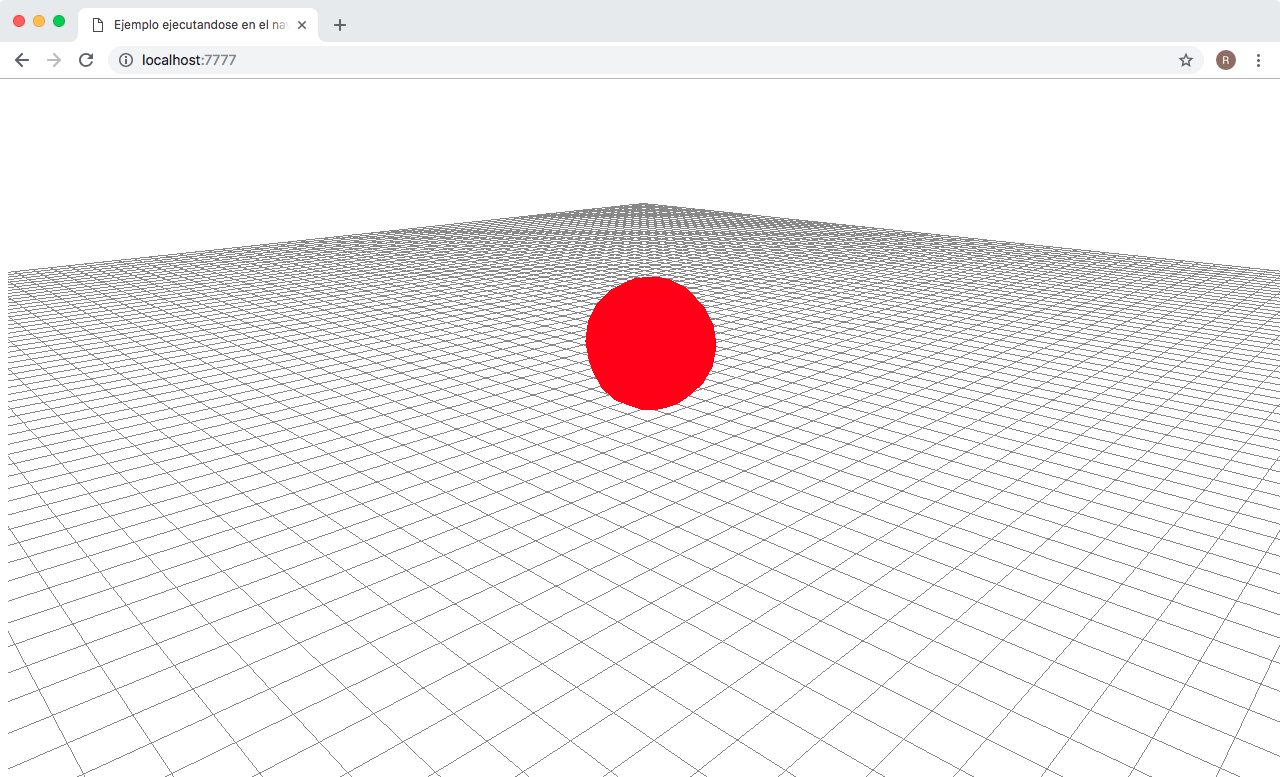
\includegraphics[width=0.8\textwidth]{figures/esferathreejs.png}
		\caption{Esfera creada con la biblioteca Three.js y mostrada en un navegador}
		\label{fig.esferathreejs}
		\end{center}
\end{figure}

\section{WebRTC}
WebRTC \footnote{\url{https://webrtc.org/}}  una tecnología que permite a una aplicación web capturar y transmitir audio y video, así como intercambiar datos audiovisuales con otros navegadores sin necesidad de intermediarios. Este intercambio se realiza de igual a igual (\textit{peer-to-peer}) sin necesidad de instalaciones o software adicionales. WebRTC proporciona varios API y protocolos interrelacionados para dar a los navegadores y aplicaciones móviles la capacidad de intercambiar elementos multimedia en tiempo real (\textit{Real Time Communications}). Esta tecnología esta soportada en los principales navegadores y tiene el soporte de Google.

En este proyecto se usa WebRTC para la adquisición del video obtenido de una cámara web. Para lograr este objetivo, se utiliza el API de WebRTC Media Stream, que proporciona la descripción de los flujos de datos de audio y video, los métodos para trabajar con ellos, la conexión con los dispositivos para adquirirlos, las limitaciones asociadas a cada tipo de datos o los eventos asociados al proceso.

\section{El entorno Electron}
Electron\footnote{\url{https://electronjs.org/docs}} es un entorno de código abierto desarrollado por GitHub. Comenzó su desarrollo en 2013, en el mismo grupo de trabajo del editor Atom\footnote{\url{https://atom.io/}}. Fue concebido con la idea de permitir la creación de aplicaciones de escritorio multiplataforma con tecnologías web. Electron es la combinación de NodeJS y Chromium\footnote{\url{https://www.chromium.org/Home}} en una misma ejecución.

La arquitectura de una aplicación que utiliza Electron está formada por dos procesos: Principal y Renderizador. 

El proceso principal es el encargado de generar la interfaz de usuario mediante la creación de páginas web y las administra de modo que es posible mostrar más de una página web al mismo tiempo. Esta labor se realiza mediante la instancia al objeto \texttt{BrowserWindow} de Electron, ejecutándose una página web cada vez que se instancia. Cuando se destruye una de estas instancias, se está cerrando esa página web. Cada aplicación con Electron debe constar de un único proceso principal, y corresponderá al \texttt{script main} del archivo \texttt{package.json}.

El proceso renderizador es cada instancia del objeto \texttt{BrowserWindow} y la ejecución de la página web correspondiente. Una aplicación con Electron puede tener multitud de procesos renderizadores, siendo cada uno independiente del resto. Cada proceso solo se preocupa de la página web que se está ejecutando en él.

Electron es totalmente compatible con NodeJS, tanto en el proceso principal como en el renderizador, por lo que todas las herramientas disponibles para Node.js, también lo están para Electron. Así mismo, es posible utilizar módulos Node.js alojados en el repositorio de paquetes \textit{npm} mencionado anteriormente. Éste nos aporta un gran número de ventajas como una mayor seguridad al cargar contenido remoto, tener siempre actualizadas las aplicaciones o tener un gran número de bibliotecas disponibles.

Todas las aplicaciones que se desarrollarán en este trabajo podrán ser ejecutadas utilizando Electron, lo que permite utilizarlas en cualquier plataforma o, incluso, empaquetarlas usando \textit{npm} o mediante un archivo Asar\footnote{\url{https://github.com/electron/asar}}.

\subsection{Adaptación de una aplicación web a Electron}

Típicamente una aplicación que utiliza Electron está formada por:

\begin{enumerate}
\item Un archivo HTML.
\item Un fichero \texttt{main.js}, que define la ventana donde se mostrará el fichero HTML y se creará.
\item El archivo \texttt{package.json}, que define la aplicación en Electron (nombre, versión, descripción, etc.), se indican en él las dependencias a módulos externos y el fichero main.js para que crear la aplicación.
\end{enumerate}
Una vez que se cuenta con estos tres elementos, se puede instalar las dependencias mediante \texttt{npm install} (igual que para Node.js) y ejecutar la aplicación mediante \texttt{npm start} o \texttt{npm test} (dependerá de como se haya definido \texttt{package.json}).

\subsubsection{package.json}
El cometido de este archivo es definir las dependencias de paquetes de terceros que tiene la aplicación web, las características de la aplicación (nombre, versión, autor, etc.) y, lo que es más importante, de qué manera se lanzará la aplicación y el archivo que se debe ejecutar al lanzarla. El cuadro 3.1 muestra un ejemplo de un archivo \texttt{package.json}
\begin{lstlisting}[frame=single]
{"name": "Ejemplo",
  "version": "0.1.0",
  "main": "main.js",
  "scripts": {
    "start": "electron ."
  },
  "dependencies": {
      "electron": "^1.8.4",
  }
}
\end{lstlisting}

Como se puede apreciar, la versión de Electron que se utilizará será la 1.8.4.

\subsubsection{main.js}
El archivo \texttt{main.js}, contiene muy pocas líneas de código al tratarse de un elemento totalmente externo a la aplicación y no tener ningún papel en su funcionamiento. Únicamente es necesario para ejecutar la aplicación utilizando Electron. El cuadro 3.2 muestra un ejemplo del contenido de este archivo.

\begin{lstlisting}[frame=single]
const app = require('electron')
const path = require('path')
const url = require('url')

let win;

function createWindow () {
  win = new BrowserWindow({width: 1800, height: 1000})
  win.loadURL(url.format({
    pathname: path.join(__dirname, 'camserver.html'),
    protocol: 'file:',
  }))
  
app.on('ready', createWindow)

\end{lstlisting}

Lo primero que se hace es definir los módulos que se requieren para que funcione correctamente y que se utilizarán en el resto del código. Posteriormente, se define el tamaño de la ventana, en este caso la ventana será de 1800 pixeles de ancho y 1000 de alto. Mediante \texttt{win.loadURL} se simula el funcionamiento de un navegador y como gestionan las diferentes URL. A este método se le pasarán como parámetros el archivo HTML principal de la aplicación web y el protocolo que este caso es \texttt{file:}, al estar queriendo mostrar directamente de un archivo HTML (si quisiéramos mostrar mediante Electron el contenido de una página web ya existente, el protocolo tomaría el valor \texttt{http:}). Finalmente, la última línea de código llamará a la función que crea la ventana y muestra el HTML en el momento que Electron haya terminado de inicializarse y está preparado para la creación de la ventana.


En la figura 3.8 se muestra el mismo HTML ejecutado con Node.js y con Electron. Como se puede apreciar, el resultado es el mismo.

\begin{figure}[H]
  \begin{center}
    \subfigure[Node.js]{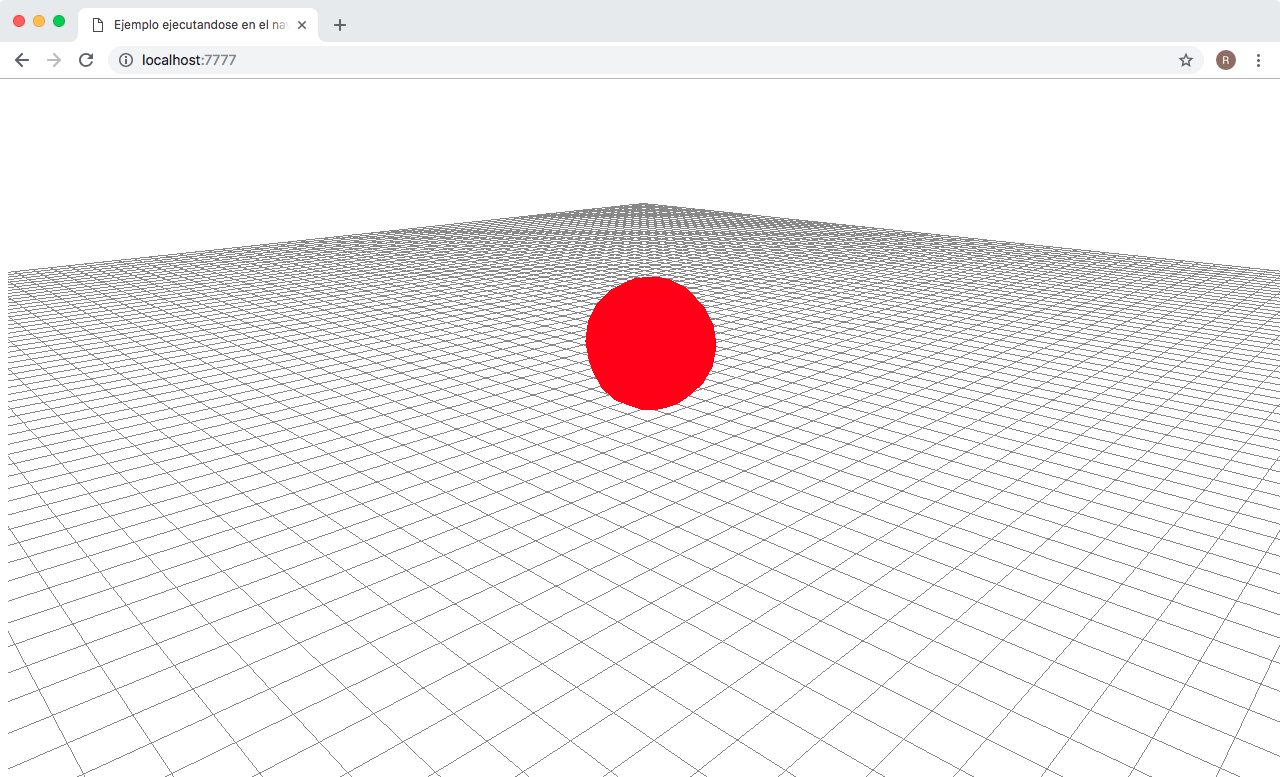
\includegraphics[width=0.4\textwidth]{figures/esferathreejs.png}}
    \subfigure[Electron]{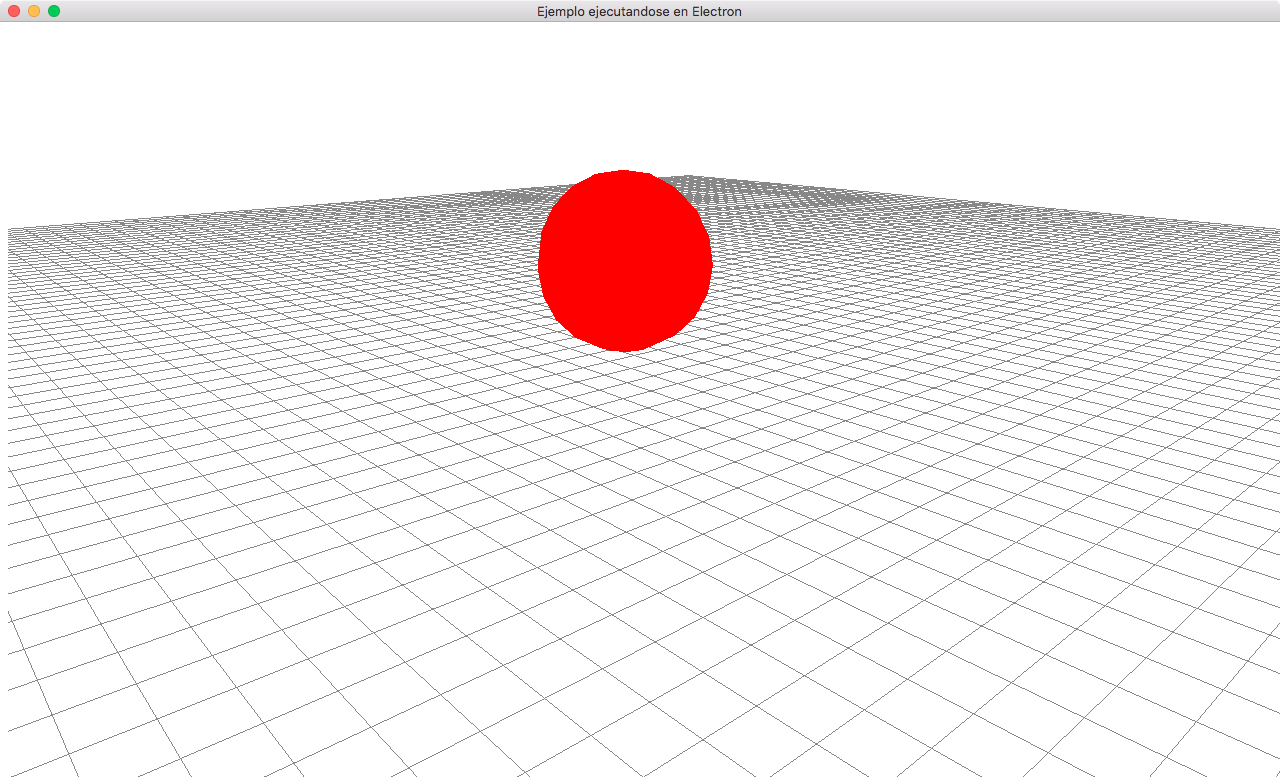
\includegraphics[width=0.4\textwidth]{figures/ejemploelectron.png}}
    \caption{Ejemplo de la esfera anterior ejecutado con Node.js y con Electron}
     \label{fig.ejemplohtmlcomm}
     \end{center}
\end{figure}






